\section{Suddivisione in Package}

La fase di progettazione ha portato ad individuare numerose classi. E` risultata fondamentale una corretta suddivisione in package, sia nel lato server che nel lato client dell'applicazione. Ogni package verr\`a analizzato singolarmente nelle varie sottosezioni.

\paragraph{BitCreekPeer}
Nel realizzare il peer abbiamo suddiviso il codice in tre package
\begin{itemize}
\item gui: contiene tutto il codice necessario per il funzionamento dell'interfaccia grafica. Vi sono degli ulteriori riferimenti alla cartella icone contenente tutte le icone utilizzate dalla GUI.
\item peer: contiene tutto il codice relativo alle politiche e ai thread del peer
\item condivisi: si tratta di un package condiviso tra peer e server
\end{itemize}
\paragraph{BitCreekServer}
Nel realizzare il peer abbiamo suddiviso il codice in tre package
\begin{itemize}
\item server: contiene tutto il codice necessario per il funzionamento del server
\item condivisi: vedi sopra
\end{itemize}
\paragraph{Condivisi}
E` un package condiviso tra peer e server, principalmente contiene tutte le classi necessarie per il funzionamento dell'RMI, gestione eccezioni e dati scambiati tra peer e server.

\subsection{server}

Il package $server$ contiene le seguenti classi:

\begin{itemize}
\item BitCreekServer: Classe principale contenente il main del server
\item ImplementazioneRMI: implementazione dei metodi presenti nell'InterfacciaRMI condivisa tra peer e server.
\item ListaPeer: ArrayList di NetRecord gestita dai Tracker del server (relativa a singolo Swarm).
\item MetaInfo: HashSet di Descrittori
\item NumPeer: Classe che tiene traccia di Seeder e Leecher (relativa a singolo Swarm).
\item ServerListener: Thread di gestione del meccanismo di aggiramento del NAT.
\item ThreadSaver: Thread di gestione del salvataggio su file della lista degli swarm presenti.
\item TrackerTCP: Thread di gestione della ricerca Peer.
\item TrackerUDP: Thread di gestione del meccanismo di Keep Alive.
\item Trimmer: Classi che implementa le funzionalit\`a di rimozione Peer che non rispondo al KeepAlive.
\end{itemize}

e sfrutta le classi presenti in $condivisi$:

\begin{itemize}
\item Descrittore: Classe che racchiude tutte le informazioni relative allo swarm.
\item ErrorException: Classe che estende le normali eccezioni in Java, utilizzata per un trattamento uniforme di tutte le eccezioni che vanno notificate all'utente.
\item InterfacciaRMI: Interfaccia condivisa con il peer per il meccanismo RMI
\item InterfacciaCallback: Interfaccia condivisa con il peer per il meccanismo delle CallBack
\item NetRecord: Classe che definisce le informazioni necessarie alla lista Peer
\item Porte: Classe wrapper utilizzata per definire le informazioni che un peer deve ricevere a seguito dell'invio di un descrittore appena creato; contiene le porte del trackerUDP e TCP associati allo swarm appena creato.
\end{itemize}

diagramma UML delle classi:

\begin{figure}[h]
  \centerline{
    \mbox{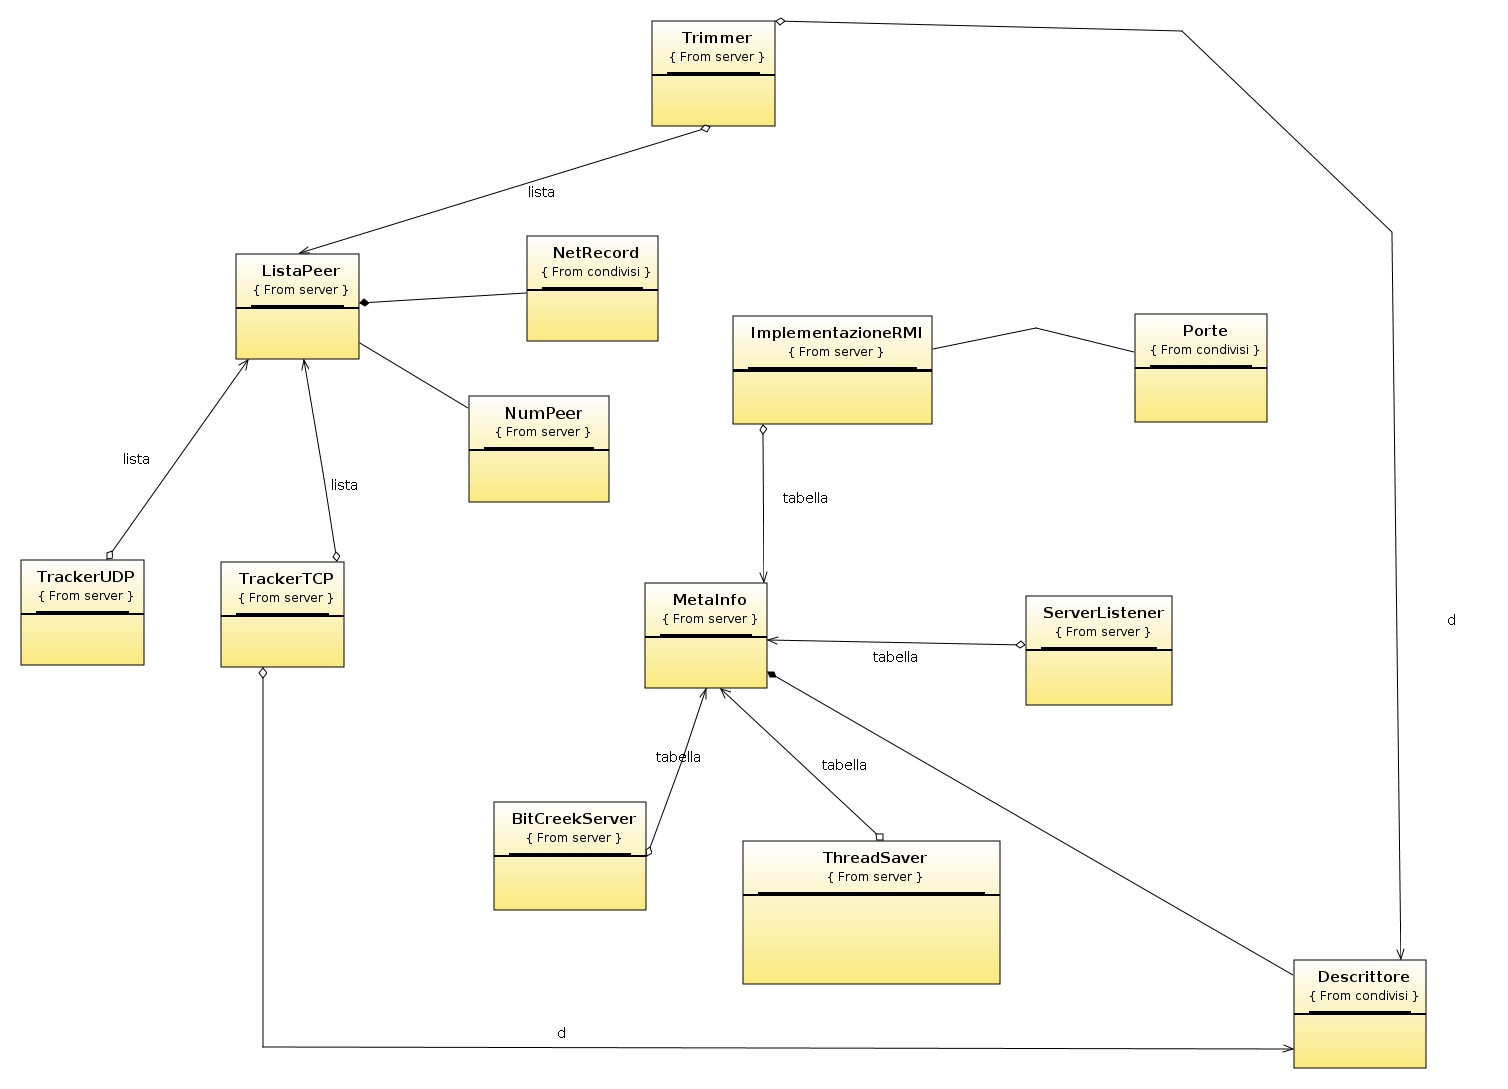
\includegraphics[scale=0.35]{images/serverClass.jpg}}
  }
  \caption{Diagramma delle classi del Server.}
  \label{classiServer}
\end{figure}

\subsection{peer}

Il package $gui$ contiene le seguenti classi:

\begin{itemize}
\item BitCreekGui: Classe principale del package, contenente il main dell'applicazione lato Peer.
\item FunctionPanel: Classe che implementa il grafico delle connessioni.
\item ModelloTabellaCerca
\item ModelloTabellaMieiCreek
\item ModelloTabellaPubblicati
\item RigaTabellaCerca
\item RigaTabellaMieiCreek
\item RigaTabellaPubblicati
\end{itemize}

Il package $peer$ contiene le seguenti classi:

\begin{itemize}
\item BitCreekPeer: Classe principale del package, viene creato da BitCreekGui al momento dell'avvio dell'applicazione.
\item Apri: Thread di apertura di un file .creek
\item Ascolto: Thread di ascolto di nuove connessioni
\item Avvia: Thread di Avvio di un nuovo swarm
\item Bitfield: Classe che definisce un messaggio di risposta a livello di HandShake applicativo.
\item Cerca: Thread che effettua una ricerca sul server.
\item Chunk: Classe che definisce tutti gli attributi di un chunk del file relativo allo Swarm.
\item Connessione: Classe che virtualizza la connessione tra 2 peer
\item Contact: Classe che definisce il primo Messaggio a livello di Hanshake Applicativo.
\item Crea: Thread che implementa la creazione di un nuovo Descrittore da submittare tramite RMI al server.
\item Creek: Classe che definisce gli attributi necessari alla gestione di uno swarm (a runtime).
\item Downloader: Thread che gestisce lo scaricamento di un file su di una connessione.
\item Elimina: Thread che gestisce l'eliminazione di un creek con relativa comunicazione al server.
\item Implementazione Callback: gestione della callback relativa alla ricerca.
\item KeepAlive: Thread che gestisce l'invio dei messaggi di KeepAlive.
\item Messaggio: Classe che definisce i messaggi scambiati tra per lo scaricamento di un file.
\item PIO: Classe che definisce gli attributi di un Chunk da scaricare.
\item Riavvia: Thread invocato al per la gestione di Swarm interrotti.
\item Uploader: Thread che gestisce l'upload su una connessione.
\item UploadManager: Thread relativo ad ogni swarm per la gestione delle politiche di upload.
\end{itemize}

Il peer utilizza le classi contenute nel package condivisi, gia illustrato nella sezione precedente.

diagramma UML delle classi:

\begin{figure}[h]
  \centerline{
    \mbox{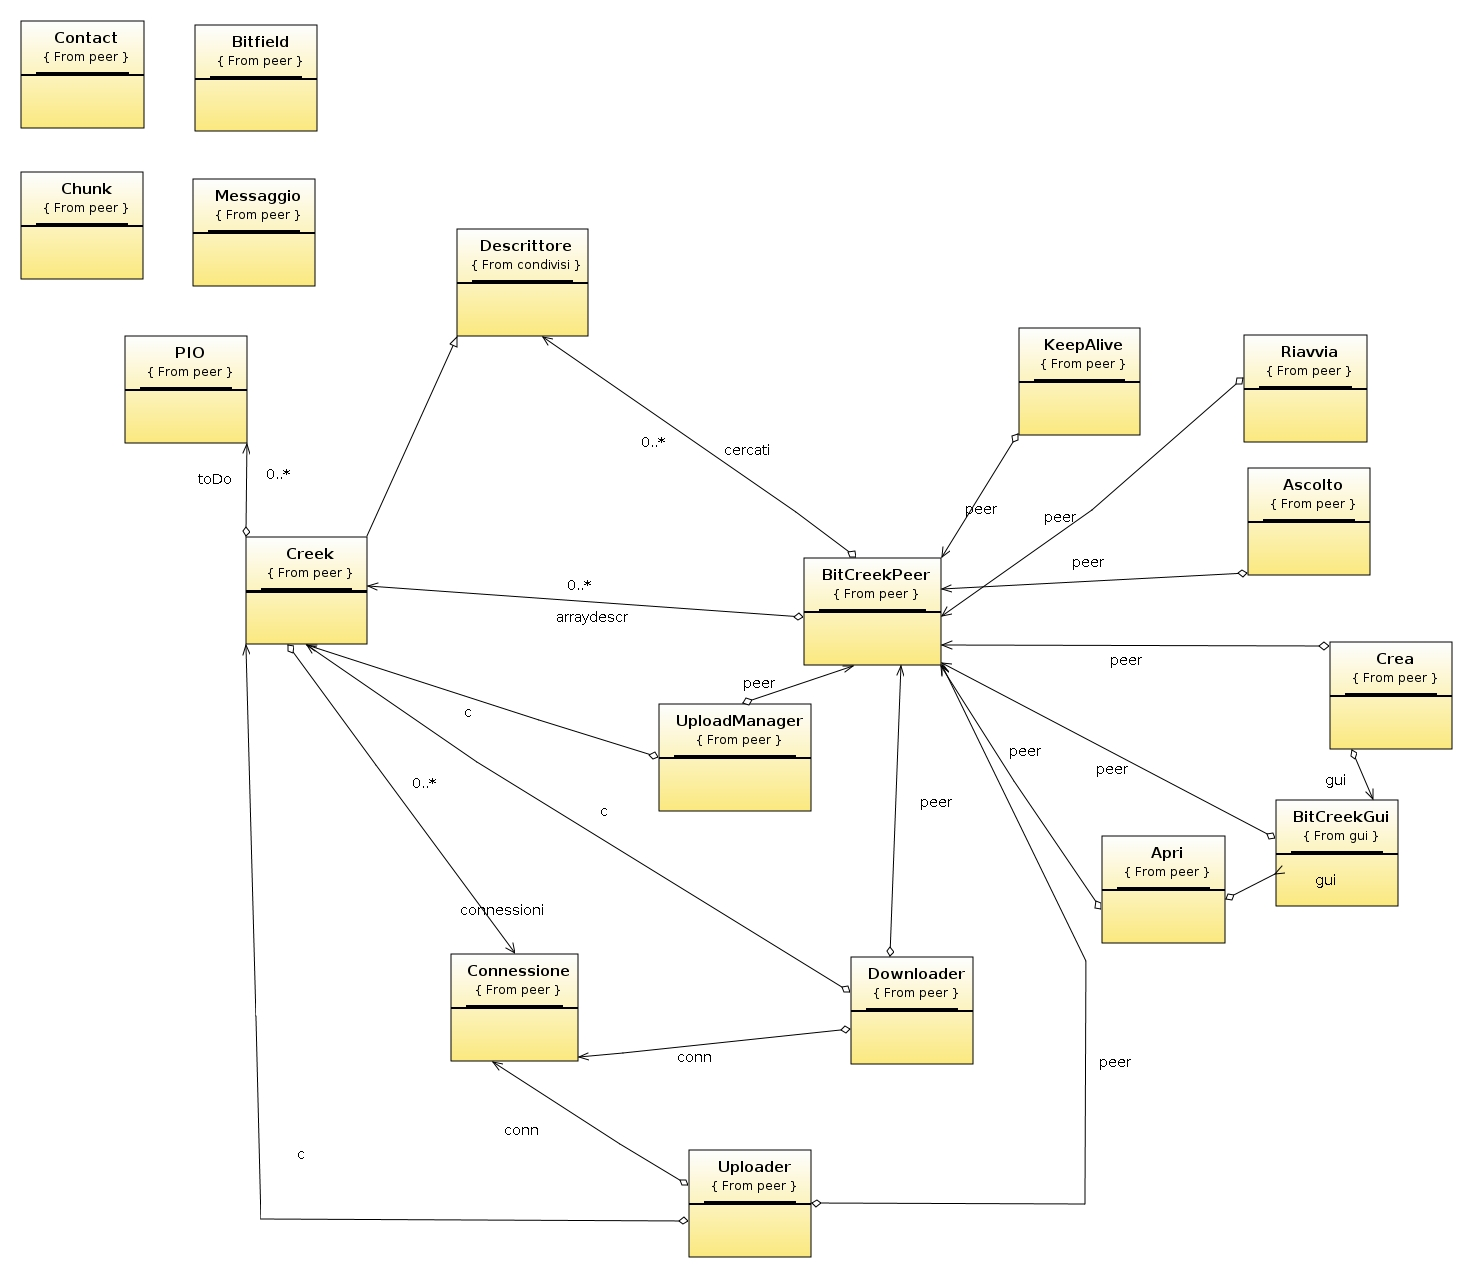
\includegraphics[scale=0.35]{images/peerClass.jpg}}
  }
  \caption{Diagramma delle classi del Peer.}
  \label{overView}
\end{figure}

